\begin{pastexam}[label={px:ccu-109-csb-01}]{中正資工所乙組 109 學年度 第 4 題}
（問答）

(10\%) Please answer the following questions for the two binary trees in the following figure.
\begin{enumerate}[label=(\alph*)]
\item (4\%) For each tree in the following figure, list the leaf nodes and the non-leaf nodes.
\item (6\%) Write out the inorder, preorder, and postorder traversals for each tree in the
following figure.
\end{enumerate}

\begin{center}
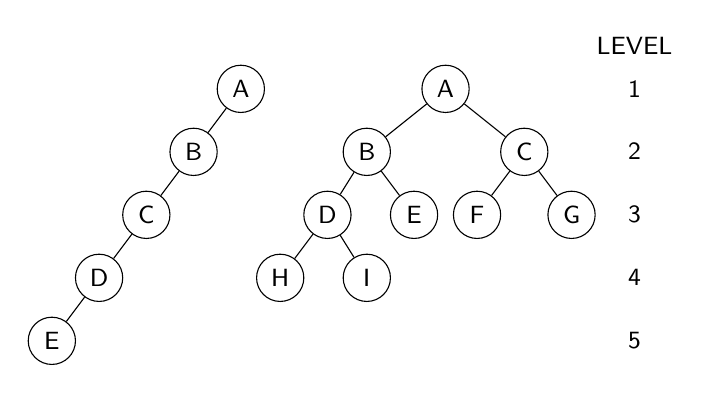
\begin{tikzpicture}[v/.style={circle,draw,minimum size=6mm,inner sep=0pt,font=\small\sffamily}]
% left tree (left-skewed)
\node[v] (a) at (0,0) {A};
\node[v] (b) at (-0.6,-0.8) {B};
\node[v] (c) at (-1.2,-1.6) {C};
\node[v] (d) at (-1.8,-2.4) {D};
\node[v] (e) at (-2.4,-3.2) {E};
\draw (a)--(b)--(c)--(d)--(e);
% right tree
\node[v] (A) at (2.6,0) {A};
\node[v] (B) at (1.6,-0.8) {B};
\node[v] (C) at (3.6,-0.8) {C};
\node[v] (D) at (1.1,-1.6) {D};
\node[v] (E) at (2.2,-1.6) {E};
\node[v] (F) at (3.0,-1.6) {F};
\node[v] (G) at (4.2,-1.6) {G};
\node[v] (H) at (0.5,-2.4) {H};
\node[v] (I) at (1.6,-2.4) {I};
\draw (A)--(B) (A)--(C) (B)--(D) (B)--(E) (C)--(F) (C)--(G) (D)--(H) (D)--(I);
% levels
\node[font=\small\sffamily] at (5.0,0.55) {LEVEL};
\foreach \l/\y in {1/0,2/-0.8,3/-1.6,4/-2.4,5/-3.2}
  \node[font=\small\sffamily] at (5.0,\y) {\l};
\end{tikzpicture}
\end{center}
\end{pastexam}

\begin{pastsoln}
左邊那棵叫 $T_1$，右邊那棵叫 $T_2$。 $T_1$ 每個節點都只有\textbf{左}子節點（圖上一路往左下），
是一棵左斜樹；用資結書第~7.1~節的文字寫法是 $T_1 = A(B(C(D(E, -), -), -), -)$，
$T_2 = A\bigl(B(D(H, I), E),\; C(F, G)\bigr)$。

\textbf{(a)} 葉節點是沒有子節點的節點，其餘是非葉節點（內部節點）。
\begin{center}
\begin{tabular}{lll}
\toprule
 & 葉節點 & 非葉節點 \\
\midrule
$T_1$ & $E$ & $A, B, C, D$ \\
$T_2$ & $H, I, E, F, G$ & $A, B, C, D$ \\
\bottomrule
\end{tabular}
\end{center}
檢查 $T_2$：分支度為 $2$ 的節點有 $A, B, C, D$ 共 $4$ 個，葉節點 $5$ 個，符合
$n_0 = n_2 + 1$（資結書定理~7.2）。

\textbf{(b)} 三種走訪的定義（資結書第~7.3~節）：中序是「左子樹、根、右子樹」，前序是「根、左、
右」，後序是「左、右、根」。

$T_1$：每個節點只有左子樹，右子樹都是空的。
\begin{itemize}
\item 中序：先走完左子樹再印根，最深的 $E$ 最先印出：$E\,D\,C\,B\,A$。
\item 前序：先印根再往左走：$A\,B\,C\,D\,E$。
\item 後序：左子樹走完才印根，右子樹是空的：$E\,D\,C\,B\,A$。 和中序相同，因為每個節點的右子樹
都是空的，「左、根、右」和「左、右、根」印出來一樣。
\end{itemize}

$T_2$：一層一層展開。 以中序為例，
\[
\mathrm{in}(A) = \mathrm{in}(B)\; A\; \mathrm{in}(C)
= \bigl(\mathrm{in}(D)\; B\; E\bigr)\; A\; \bigl(F\, C\, G\bigr)
= (H\,D\,I)\; B\; E\; A\; F\; C\; G .
\]
\begin{itemize}
\item 中序：$H\,D\,I\,B\,E\,A\,F\,C\,G$。
\item 前序：$A\,(B\,(D\,H\,I)\,E)\,(C\,F\,G) = A\,B\,D\,H\,I\,E\,C\,F\,G$。
\item 後序：$((H\,I\,D)\,E\,B)\,(F\,G\,C)\,A = H\,I\,D\,E\,B\,F\,G\,C\,A$。
\end{itemize}
\end{pastsoln}
